In this section, we provide the necessary background from a control theory perspective to facilitate the understanding of the remainder of this work. Initially, we introduce general concepts related to optimization problems. Subsequently, we delve into the foundational principles of Nonlinear Programming (NLP), with a focus on Nonlinear Model Predictive Control (NMPC) and its application within control loops. Finally, we explore the concept of cooperative control and its relevance to multiagent systems.

\subsubsection{Optimization Problems}

An optimization problem is defined as the task of determining the best, or optimal, solution among all feasible solutions while adhering to a set of constraints. This process typically involves minimizing an objective function, often referred to as the cost function in specific applications. For cases where maximization is desired, the problem needs to be reformulated to minimize the negative of the cost function.

The general formulation of an optimization problem presented in \ref{eq:optimization_problem_with_soft_constraint}. In this formulation, \( f(x) \) represents the cost function, \( x \) denotes the decision variables, \( e_i(x) \) corresponds to equality constraints, and \( g_j(x) \) represents inequality constraints. Constraints such as \( e_i(x) = 0 \) and \( g_j(x) \geq 0 \) are referred to as hard constraints, meaning they must always be strictly satisfied. However, in certain situations, strict enforcement of constraints can render the optimization problem infeasible, especially when the constraints cannot always be satisfied due to problem-specific limitations.

To address this issue, a soft constraint term, \( sc(x) \), is introduced into the cost function. Unlike hard constraints, soft constraints do not require strict satisfaction; instead, they penalize violations within the objective function. This provides flexibility and ensures that the problem remains solvable even when some constraints cannot be strictly adhered to. The inclusion of \( sc(x) \) is particularly useful in scenarios where feasibility might otherwise be impossible with hard constraints alone.

\begin{equation}
    \begin{aligned}
        &\underset{x}{\text{minimize}} \quad f(x) + sc(x) \\
        &\text{subject to}\\
        &\quad \quad e_i(x) = 0, \quad i = 1, \dots, m, \\
        &\quad \quad \, g_j(x) \geq 0, \quad j = 1, \dots, p.
    \end{aligned}
    \label{eq:optimization_problem_with_soft_constraint}
\end{equation}

After introducing the general concept of optimization problems, Sequential Quadratic Programming (SQP) can be presented as an effective method for solving nonlinear optimization problems. SQP is particularly suitable for problems with constraints, as it approximates the original nonlinear problem by iteratively solving quadratic programming (QP) subproblems. Each subproblem optimizes a quadratic approximation of the cost function while maintaining a linearized version of the constraints.

SQP leverages second-order information about the problem, such as the Hessian of the Lagrangian, making it a powerful approach for problems requiring high accuracy. By solving the sequence of QP subproblems, SQP ensures that both the objective function and constraints are handled efficiently, even for highly nonlinear formulations.

\subsubsection{Nonlinear Model Predictive Control}

Nonlinear Model Predictive Control (NMPC) is an optimization-based technique for the feedback control of nonlinear systems, incorporating system constraints \cite{grune2017nonlinearmpc}. In order to use this technique, we need to first derive a discretized model of the system in use, since this will be necessary to predict the behavior of the system during the desired horizon. After this we solve we compute the optimal control input with relation to the chosen cost function during a certain horizon, but we use only the first control input. The optimization process is then repeated in the next time step.

As illustrated in Figure \ref{fig:simplified_mpc_control_loop}, NMPC operates as a closed-loop control system, using the current state of the system as an input. This ensures that any deviations from the system model are accounted for in subsequent iterations.

\begin{figure}[h]
    \centering
    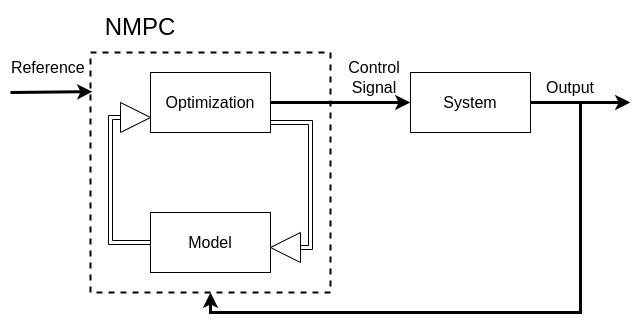
\includegraphics[width=0.8\textwidth]{Images/Background/MPC/NMPC.jpg}
    \caption{Simplified Block Diagram of an NMPC Controller}
    \label{fig:simplified_mpc_control_loop}
\end{figure}

The internal mechanism of Model Predictive Control (MPC), whether linear or nonlinear, follows the same fundamental principles~\cite{grune2017nonlinearmpc,schwenzer2021review}. 
A summary of the NMPC workflow for each time step \( t = 1, 2, \dots \) is as follows:


\begin{itemize}
    \item \textbf{State Measurement:} Measure the current state of the system, \( x(s) \in \mathbb{X} \), where \( \mathbb{X} \) is the system's state space.
    \item \textbf{Optimization Problem Definition:} We formulate the optimal control problem (OCP) as shown in \ref{eq:mpc_optimization_problem} over a horizon with dimension \( N \), where \( x(k) \) and \( u(k) \) represent the state and control signal at time \( k \) respectively. \(x_0\) represent the measured initial state of the system. The function \( f \) represents the system dynamics model, meaning with input \( x(k) \) and \( u(k) \) we compute as state at time \( k + 1 \), allowing us to predict the behavior of the system during the horizon. The function  \( l \) maps the state and control signal at time  \( k \) to a scalar value, representing the cost function we want to minimize, and \( J \) represent the cost over the full horizon. The sets \( \mathbb{X} \) and \( \mathbb{U} \) contain all the valid values for the state and control signal, respectively.
    
    \begin{equation}
        \begin{aligned}
            &\underset{u(\cdot) \in  \mathbb{U}^{N}(x_{0})}{\text{minimize}} \quad J_{N}(x_{0}, u(\cdot)) = \sum_{k=0}^{N-1} l(x(k, x_0), u(k)) \\
            &\text{subject to} \quad x(0) = x_0, \\
            &\quad \quad \quad \quad x(k+1) = f(x(k), u(k)) \\
            &\quad \quad \quad \quad x(k), \in \mathbb{X} \quad k = 0, \dots, N-1\\
            &\quad \quad \quad \quad u(k) \in \mathbb{U}, \quad k = 0, \dots, N-1.
        \end{aligned}
        \label{eq:mpc_optimization_problem}
    \end{equation}
    \item \textbf{Feedback and Update:} Use the computed NMPC feedback value \\ \( \mu_{N}(x(n)) := u(0) \) for control until the next sampling period. Remaining control values can be discarded or used as warm-start inputs for the next optimization iteration.
\end{itemize}

NMPC systems often consider two types of horizons, as discussed in \cite{schwenzer2021review}: the \textit{prediction horizon} \( N_p \), where future system dynamics are simulated, and the \textit{control horizon} \( N_c \), where optimal control inputs are computed. For simplicity, we assume \( N_c = N_p \), however in the special case that \( N_c < N_p \), the control input is held constant for the remaining steps.

\paragraph{Real time iteration scheme} first proposed in~\cite{diehl2002real}, is a common way to reduce the time taken in the controller, making it easier to run in a real time, where sometimes the max computation time is in the order of milliseconds. In this schema we compute only 1 SQP iteration per time step, and divided computation into two different phases, preparation and feedback. All operation that are not depended on the knowledge of the current state, are included in the preparation phase, since they can be executed offline, reducing the load during the online phase. The feedback phase starts when we measure the current state, we then construct the QP problem and solved it, receive as solution not the u and x, but rather us a $\Delta u$ and $\Delta x$. With this we can compute the control input as $u = u_{guess} + \Delta u$, where the $u_{guess}$ is the initial guess passed to the solver, we then apply this value for a certain time interval, during which the preparation phase is being executed as per~\cite{diehl2005real}. We then use the current $x$ and $u$ as the next iteration phase initial guess, reducing the cost of the next iteration. 

\subsubsection{Distributed NMPC}

Distributed NMPC is an extension of NMPC~\cite{muller2013distributed}, where a large complex problem is decomposed into multiple smaller subproblems that can be solved individually. Each individual controller solves its local problem while coordinating with others to ensure consensus is reached for the values of global variables. This approach is particularly useful in multiagent systems, where each agent solves its own problem while the global problem is addressed through coordination and consensus. By solving multiple smaller problems instead of one large problem, the computational burden is reduced, although the overall architecture becomes more complex. Consensus is typically achieved by computing the average of shared variables and using this new value as the start value for the next iteration, with convergence determined when the maximum difference between the variables and the average falls below a certain threshold. The Alternating Direction Method of Multipliers (ADMM)~\cite{boyd2011distributed} is commonly used to facilitate this consensus by iteratively solving local subproblems and enforcing consistency through penalty terms and dual variable updates.